%!TEX root = ../thesis.tex
%*******************************************************************************
%****************************** Third Chapter **********************************
%*******************************************************************************

\newtheorem{theorem}{Theorem}[section]
\newtheorem{corollary}{Corollary}[theorem]
\newtheorem{lemma}[theorem]{Lemma}
\newtheorem{definition}{Definition}[section]

\chapter{Feynman-Kac: connecting Quantum Mechanics and Stochastic Processes}
\label{chapter3}

% **************************** Define Graphics Path **************************
\ifpdf
    \graphicspath{{Chapter3/Figs/Raster/}{Chapter3/Figs/PDF/}{Chapter3/Figs/}}
\else
    \graphicspath{{Chapter3/Figs/Vector/}{Chapter3/Figs/}}
\fi
In this chapter we will provide a bridge between the quantum many-body problem discussed in the previous chapter and stochastic processes. This will entail introducing the Feynman-Kac formula and relating it to the Fokker-Planck equation and optimal control approaches to QM. Moreover, a probabilistic view of the cost function will lead us to proposals for loss functions that can be used to learn optimal transition rates and consequently sample the ground state.

The field of stochastic processes is a vast body of work, approached from different angles by mathematicians, physicists and engineers. A necessary consequence of this is that the literature ranges from extremely thorough and rigorous~\cite{rogers1994diffusions, rogers2000diffusions} to more applied and intuitive~\cite{sarkka2019applied}. For this reason, the mentioned discussion will be preceded by an overview of the mathematical notation, lemmas and results from stochastic processes and measure theory that underpin some core ideas of this thesis. To avoid including a whole textbook of material on measure and stochastic processes some concepts will not be rigorously defined, the text will point to relevant literature where this is the case.

\section{Stochastic processes}
\label{subsec:fk-stoch}
\subsection{Fundamentals}
This brief, more formal, discussion of stochastic processes is based mostly upon classic texts~\cite{durrett2019probability, rogers1994diffusions, rogers2000diffusions} and borrows some intuitions from~\cite{sarkka2019applied}. The most basic quantity that we will need is the \textbf{probability space}. 
\begin{definition}[Probability space]
	The probability space is a tuple $(\Omega, \mathcal{F}, \mathbb{P})$, where $\Omega$ is the \textbf{sample space}, $\mathcal{F}$ is a $\sigma$-\textbf{field}, and $\mathbb{P}$ is the \textbf{measure}.
\end{definition}
The sample space is simply the set of all possible outcomes. A canonical example would be the roll of a 6-sided dice, $\Omega=\{1, 2, 3, 4, 5, 6\}$. Without measure $\mathbb{P}$, the tuple $(\Omega, \mathcal{F})$ is termed a \textbf{measurable space}.
\begin{definition}[$\sigma$-field]
	A $\sigma$-field $\mathcal{F}$ on a set $\Omega$, is a nonempty collection of subsets of $\Omega$ that includes $\Omega$ itself, is closed under complement, i.e. if $A \in \mathcal{F}$ then $A^c \in \mathcal{F}$, and is closed under countable unions, $\cup_{i} A_{i} \in \mathcal{F}$ if $A_{i} \in \mathcal{F}$ is a countable union of sets.
\end{definition}
The main utility of the $\sigma$-field to us is its use in defining measures. We want to be able to assign a non-negative real number to all subsets of $\Omega$, as well as the size of the union of the disjoint sets to be the sum of their individual sizes. This is not always possible, a counterexample for the real line being Vitali sets. The collection $\mathcal{F}$, must thus only include \emph{measurable} sets, which are precisely the ones that satisfy the constraints imposed by the $\sigma$-field.
\begin{definition}[Measure]
	A non-negative countably additive set function $\mu: \mathcal{F} \rightarrow \mathbb{R}$ that satisfies
	\begin{enumerate}[label=\roman*)]
		\item $\mu(A) \geq \mu(\emptyset)=0$ for all $A \in \mathcal{F}$
		\item if $A_{i} \in \mathcal{F}$ is a countable sequence of disjoint sets, then $\mu\left(\cup_{i} A_{i}\right)=\sum_{i} \mu\left(A_{i}\right)$
	\end{enumerate}
	is a \textbf{measure}.
\end{definition}
If $\mu(\Omega)=1$, then $\mu$ is a \textbf{probability measure} and will be denoted by $\mathbb{P}$. With this notion we are now able to define a random variable (r.v) and a stochastic process (s.p.).
\begin{definition}[Random variable]
	 A \textbf{random variable} $X$ defined on $\Omega$ is a real-valued measurable function $X(\omega)$, $X: \Omega \rightarrow \mathbb{R}^d$.
\end{definition}
For a function to be measurable, we require that its preimage $X^{-1}$ is in the $\sigma$-field $\mathcal{F}$
\begin{equation}
	X^{-1}(B) = \{ \omega : X(\omega) \in B \} \in \mathcal{F},
\end{equation}
and that this holds for every Borel set $B$ in the Borel $\sigma$-field~\footnote{For a proper definition of the Borell set see ch. 3 of~\cite{salamon2016measure}.} of $\mathbb{R}^d$, which is simply the smallest $\sigma$-field that contains all measurable sets in $\mathbb{R}^d$. 

A random variable $X$ induces a probability measure $\mu$ on $\mathbb{R}^d$ called its \textbf{distribution}, this is done by setting $\mu(A)=P(X \in A)$ for Borel sets $A$. Moreover, the distribution is usually given in terms of a \textbf{distribution function} $F(x)$
\begin{equation}
	 F(x) = \mathbb{P}(\{\omega \in \Omega: X(\omega) \leq x\}) = \mathbb{P}(X \leq x),
\end{equation}
and $X$ is said to have a \textbf{density function} $f(x)$ if $F(x)$ can be written as 
\begin{equation}
	\label{eq:pdf}
	F(x)=\int_{-\infty}^{x} f(y) \mathrm{d}y. 
\end{equation}
In essence, the random variable provides a connection between the less familiar probability measure $\mathbb{P}$ and the cumulative distribution function (CDF).

\subsection{Stochastic process}
\begin{definition}[Stochastic process]
		Given a probability space $(\Omega, \mathcal{F}, \mathbb{P})$ and a measurable (state) space $(E, \mathcal{E})$, we define the collection $\left\{X_{t}: t \in T\right\}$ of set $T$ indexed and $(E, \mathcal{E})$ valued random variables a \textbf{stochastic process}.
\end{definition}
By far the most common case for the index set $T$, is time $T = \mathbb{R}^+$. Such s.p's are called \emph{temporal}, examples include the model of velocity of a Brownian particle under influence of friction, in Fig.~\ref{fig:sp-brown}, or the Black-Scholes model. Nevertheless, the index set is not limited to time, as is often the case with Gaussian Process regression~\cite{rasmussen2006gaussian}. In this thesis we will mostly deal with temporal s.p's of the kind that do not "see into the future". This notion is formalized using \textbf{filtrations}. A filtration $\mathbb{F}=\left(\mathcal{F}_{t}\right)_{t \in T}$ on a probability space $(\Omega, \mathcal{F}, \mathbb{P})$ is just an increasing sequence or order of $\sigma$-fields
\begin{equation}
	\mathcal{F}_{s} \subset \mathcal{F}_{t} \text { if } 0 \leq s \leq t<\infty
\end{equation}
The filtration associated to a process that records its "past behaviour" at each time is called the \textbf{natural filtration}. 
\begin{definition}[Adapted process]
	A process $\{X_t\}$ is said to be \textbf{adapted to the filtration} $\left(\mathcal{F}_{t}\right)_{t \in T}$ if the random variable $X_t : \Omega \rightarrow E$ is $\mathcal{F}_t$-measurable function for each $t \in T$. 
\end{definition}
A process that is \emph{non-anticipating}, i.e. depends only on the past and present, is adapted to the filtration $\left(\mathcal{F}_{t}\right)_{t \in T}$.
\begin{definition}[Brownian motion]
	\textbf{Brownian motion} or a non-anticipating \textbf{Wiener process} is a stochastic process $W_t$, with the following properties:
	\begin{enumerate}[label=\roman*)]
		\item $W_0 = 0$
		\item $W_t$ is almost surely continuous in t
		\item $W_t$ has independent increments
		\item $W_t - W_s \sim \mathcal{N} (0, t-s)$ for $0 \leq s \leq t$
	\end{enumerate}
\end{definition}
A realisation of Brownian motion can be found in Fig.~\ref{fig:sp-brown}.
\begin{figure}[h]
	\centering
	\subfloat{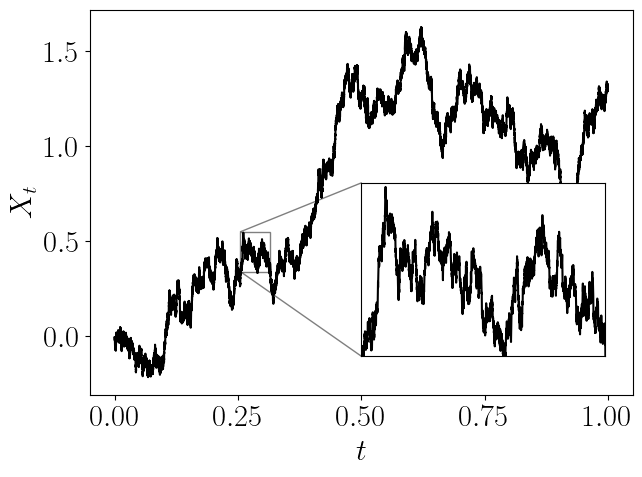
\includegraphics[width=0.5\linewidth]{Chapter3/Figs/Raster/OU-BM-I.png}}
	\subfloat{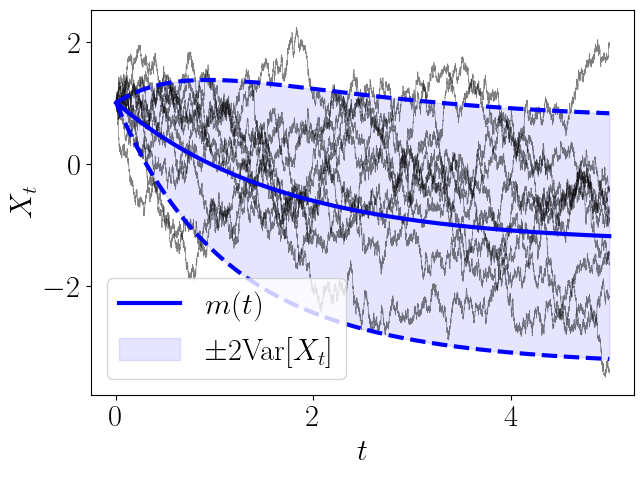
\includegraphics[width=0.5\linewidth]{Chapter3/Figs/Raster/OU-BM-II.png}}
	\caption[Brownian motion and Ornstein–Uhlenbeck process
	]{\textbf{Brownian motion and Ornstein–Uhlenbeck process.} 
		\textbf{left:} A single realisation of the Brownian process. \textbf{right:} Mean, variance and 10 samples of the Ohrnstein-Uhlenbeck process with $\theta=0.6, \sigma=1.1, X_0=1.0, \mu=-1.3$, integrated using Euler-Maruyama method.}
	\label{fig:sp-brown}
\end{figure}

\subsection{Integrals}
In order to proceed and define stochastic differential equations (SDE's) and the Radon-Nikodyn derivative, we must spend some time discussing various integrals we will use. In particular, alongside the usual Riemann integral, we will need three more types of integrals, which we will briefly describe without mathematical derivation. The simplest kind of integral we will introduce is the integral of a stochastic process
\begin{equation}
	I = \int_{0}^{t} X_t \mathrm{d}t.
\end{equation}
The simple appearance of the integral is deceiving as the integrand is a realisation of a $\mathcal{F}_t$-adapted stochastic process $\{X_t\}: \Omega \times T \rightarrow \mathbb{R}^{d}$, meaning that $I$ itself is a random variable. However, since each realisation of $X_t$ is almost surely continuous, $I$ can be expanded as a Riemann sum, which converges under mean-squared norm to $I$, so long as the mean $\mathbf{m}(t) = \mathbb{E}[X_t]$ and covariance $\textbf{k}(t,s) = \operatorname{Cov}(X_t, X_s)$ are continuous. In practice, computing the mean and covariance of $I$ is usually enough to understand the resulting stochastic process. Importantly, integrals of continuous functions of s.p's $h(X_t),~ h: \mathbb{R} \rightarrow \mathbb{R}$ can be computed in a similar manner.

The second type of integrals we need to consider, are integrals with respect to a s.p, known as \textbf{It\^ o integrals}
\begin{equation}
	\label{eq:ito}
	Y_t = \int_{0}^{t} H_s \mathrm{d}X_s,
\end{equation}
where both $H_s$ and $X_s$ are stochastic processes. The result integral $Y_t$ is itself a stochastic process which resides in the probability space $(\Omega, \mathcal{F}, \mathbb{P})$, filtered by $\left(\mathcal{F}_t\right)_{t\in T}$. The integral can be formalised by putting slight constraints on what sort of stochastic processes $X_s$ and $H_t$ can be, expanding $Y_t$ as a Riemann sum and proving convergence. Details of this procedure can be found in~\cite{rogers2000diffusions}.

Finally we must define the \textbf{Lebesgue-Stieltjes integral}~\cite{halmos2013measure}, which we need to properly define expectations of stochastic processes. 
\begin{definition}[Lebesgue-Stieltjes Integral]
		Given probability space $(\Omega, \mathcal{F}, \mathbb{P})$ and measurable function $f:\Omega \rightarrow \mathbb{R}$, the \textbf{Lebesgue-Stieltjes integral} 
		\begin{equation}
			I = \int_A f(x) \mathrm{d}\mathbb{P}(x),
		\end{equation}
		is the Lebesgue integral~\footnote{For proper definition of the Lebesgue integral see ch. 1 of~\cite{salamon2016measure}.} with respect to measure $\mathbb{P}$, $A \in \mathcal{F}$.
\end{definition}
With it we can define expectations in the probability space $(\Omega, \mathcal{F}, \mathbb{P})$ as
\begin{equation}
	\underset{{\mathbb{P}}}{\mathbb{E}}[f(x)]=\int_{\Omega} f(x) d \mathbb{P}(\boldsymbol{x}).
\end{equation}
For a newcomer to stochastic processes this formulation may seem redundant, can we not just calculate expectations using a Riemann integral and the PDF? We can, and when the distribution $\mathbb{P}$ can be expressed in terms of the PDF~\eqref{eq:pdf}, the Lebesgue integral can be interpreted in this way. However, stochastic processes need not admit a PDF, that is when the Lebesgue-Stieltjes integral is necessary.
%\begin{equation}
%	\int_{\Omega} f(x) \mathrm{d} \mathbb{P}(x)=\int_{\Omega} f(x) p(x) d \lambda(x)
%\end{equation}
\subsection{Stochastic Differential Equations}
In this thesis we will refer to a SDE as an informal notation of an It\^ o integral equation or \textbf{It\^ o process}. 
\begin{definition}[It\^ o process]
	Given deterministic functions $v: \mathbb{R}^{d} \times \mathbb{R}^{+} \rightarrow \mathbb{R}^{d}$ and $\sigma: \mathbb{R}^{d} \times \mathbb{R}^{+} \rightarrow \mathbb{R}^{d \times d}$, we define the \textbf{It\^ o process} $X_t$ as the sum of It\^ o and Lebesgue integrals
	\begin{equation}
		\label{eq:ito-process}
		X_{t+s}-X_{t}=\int_{t}^{t+s} \sigma\left(X_{u}, u\right) \mathrm{d} W_{u} + \int_{t}^{t+s} v\left(X_{u}, u\right) \mathrm{d} u,
	\end{equation}
	where $W_t$ is a Brownian motion.
\end{definition}
In simplified notation we can write~\eqref{eq:ito-process} as
\begin{equation}
	\mathrm{d} X_t = \sigma \left(X_{t}, t\right)\mathrm{d}W_t + v\left(X_{t}, t\right) \mathrm{d}t,
\end{equation}
this is what we refer to as an SDE, an example can be found in Fig.~\ref{fig:sp-brown}. The functions $v$ and $\sigma$, we will refer to as the \textbf{drift} and \textbf{volatility} of the It\^ o process respectively. The most intuitive interpretation of a SDE is in terms of the time evolution of the PDF of the process $X_t$. It is described by the \textbf{Fokker-Planck equation}~\footnote{Derivation in~\cite{sarkka2019applied}.} 
\begin{equation}
	\frac{\partial p(\mathbf{x}, t)}{\partial t}=
	-\sum_{i=1}^{N} \frac{\partial}{\partial x_{i}}\left[\mu_{i}(\mathbf{x}, t) p(\mathbf{x}, t)\right]
	+\sum_{i=1}^{N} \sum_{j=1}^{N} \frac{\partial^{2}}{\partial x_{i} \partial x_{j}}\left[D_{i j}(\mathbf{x}, t) p(\mathbf{x}, t)\right],
\end{equation}
where $p(\mathbb{x}, t)$ is the PDF of the solution to the SDE and $\mathbf{D}=\frac{1}{2} \boldsymbol{\sigma} \boldsymbol{\sigma}^{\top}$ is the diffusion tensor. Finally we state without proof a consequence of It\^ o calculus, most commonly named \textbf{It\^ o's rule} or \textbf{lemma}, it is the stochastic calculus equivalent of the chain rule
\begin{lemma}[It\^ o's lemma]
	Given an It\^ o process $X_t$ as given by ~\eqref{eq:ito-process} and a twice differentiable scalar function $f(X_t, t)$, then the It\^ o process for $f$ is
	\begin{equation}
		\mathrm{d} f = \frac{\partial f}{\partial t}\mathrm{d}t + \sum_i \frac{\partial f}{\partial x_i} \mathrm{d}x_i + \frac{1}{2}\sum_{ij} \frac{\partial^{2}}{\partial x_{i} \partial x_{j}} f \mathrm{d}x_i \mathrm{d}x_j,
	\end{equation}
\end{lemma}
when compared to ordinary calculus we notice an additional quadratic term.

\subsection{Radon-Nikodym Derivative and Girsanov theorem}
To perform importance sampling we perform a change of measure in an integral
\begin{equation}
	\int_{A} f(x) \mathrm{d} \mathbb{P}(x)=\int_{A} f(x) \frac{\mathrm{d} \mathbb{P}}{\mathrm{d} \mathbb{Q}}(x) \mathrm{d} \mathbb{Q}(x).
\end{equation}
The function that measures the rate of change of density of one measure w.r.t another is the \textbf{Radon-Nikodym derivative} $\frac{\mathrm{d} \mathbb{P}}{\mathrm{d} \mathbb{Q}}(x)$.

\begin{theorem}[Radon-Nikodym theorem]
	Let $\mathbb{P}$ and $\mathbb{Q}$ be probability measures on the measurable space $(\Omega, \mathcal{F})$, then the measurable function \textbf{Radon-Nikodym derivative} $\frac{\mathrm{d} \mathbb{P}}{\mathrm{d} \mathbb{Q}}(x): \Omega \rightarrow[0, \infty)$ exists and 
	\begin{equation}
		\mathbb{P}(A)=\int_{A} \frac{\mathrm{d} \mathbb{P}}{\mathrm{d} \mathbb{Q}}(x) \mathrm{d} \mathbb{Q}(x),
	\end{equation}
	for set $A \subseteq \mathcal{F}$.
\end{theorem}
The RN derivative will also be useful in defining the KL divergence between two \textbf{path measures}. Properly defining the path measure would bring a lot of notational overhead, it is enough to think of it as a measure on the \textbf{path space}, i.e all possible paths of a SDE, for rigour see~\cite{leonard2014pathmeasure}. 
Finally, we state the \textbf{Girsanov theorem} that is often used for transforming or removing drift functions of SDE, it is the RN derivative between an It\^ o process and one with $v = 0$ and $\sigma = 1$, i.e. Brownian motion. 
\begin{theorem}[Girsanov Theorem]
	Given It\^ o process
	\begin{equation}
		\mathrm{d}X_t = \mathrm{d}W_t + v(X_t, t)\mathrm{d}t \quad \text{and} \quad X_0 = 0 \\
	\end{equation}
	and Brownian motion $\mathrm{d}Y_t = \mathrm{d}W_t$, the RN derivative of their respective path measures $\mathbb{P}$ and $\mathbb{P}_0$	is
	\begin{equation}
		\frac{\mathrm{d} \mathbb{P}}{\mathrm{d} \mathbb{P}_0}=
		\exp \left(
		-\frac{1}{2} \int_{0}^{t}\left|v(X_s, s)\right|^{2} \mathrm{d} s+\int_{0}^{t} v(X_s, s)^{\top} \mathrm{d} W_s\right)
	\end{equation}
\end{theorem}
This \emph{change in dynamics} as we will call it later is true in the sense, that expectations for an arbitrary functional $h(\cdot)$ of the path from $0$ to $t$ are
\begin{equation}
	\label{eq:girsanov_consequence}
	\underset{\mathbb{P}_0}{\mathbb{E}}\left[h(X_t)\right] = \underset{\mathbb{P}_0}{\mathbb{E}}\left[\frac{\mathrm{d} \mathbb{P}}{\mathrm{d} \mathbb{P}_0} h(Y_t)\right]. 
\end{equation}
For a more general case and proof see~\cite{sarkka2019applied}.

\subsection{Markov processes}
We now shift our view to a special kind of s.p's, ones that satisfy the \textbf{Markov property} called \textbf{Markov processes} or \textbf{Markovian}. The property is sometimes referred to as \emph{memorylessness}, as the future of a Markov process depends only on the present state. We can classify the processes based on the system's \textbf{state-space} $S$, which can be either discrete (countable) or continuous, and the \textbf{time indexing} of the system, either discrete-time $\{X_n\}_{n \geq 0}$ or continuous-time $\{X_t\}_{t \geq 0}$. A taxonomy is given in Table~\ref{tab:MP-taxonomy}. We will not specifically discuss Markov processes in continuous state-space, but it is important to note that any It\^ o process with time-homogenous drift $v = v(X_t)$ and volatility $\sigma = \sigma(X_t)$ is Markovian.

From now on we refer to Markov processes in countable state-space as \textbf{Markov chains}. We base our discussion on~\cite{rogers1994diffusions} and~\cite{norris1998markov}. 
\begin{table}[h]
	\begin{center}
		\caption[Taxonomy of Markov processes]{\textbf{Taxonomy of Markov processes}}
		\label{tab:MP-taxonomy}
		\begin{tabular}{p{2cm}|p{6cm}|p{6cm}}
%			\toprule % <-- Toprule here
			 & Countable state-space & Continuous state-space\\
			\midrule
			Discrete time 
			&\parbox{5cm}{\textbf{index: }$\{X_n\}_{n \geq 0}$, $n \in \mathbb{Z}^{+}$ \\ \textbf{state-space: } countable set $I$ \\ \textbf{define: } stochastic $\{P\}_{ij}$ \\ \textbf{example:} DTMC}  
			&\parbox{5cm}{\textbf{index: }$\{X_n\}_{n \geq 0}$, $n \in \mathbb{Z}^{+}$ \\ \textbf{state-space: } general state-space $\Omega$ \\ \textbf{define: } stochastic kernel $K$ \\ \textbf{example:} Harris Chain}\\
			\midrule
			Continuous time 
			&\parbox{5cm}{\textbf{index: }$\{X_t\}_{t \geq 0}$, $t \in \mathbb{R}^{+}=[0, \infty)$ \\ \textbf{state-space: } countable set $I$ \\ \textbf{define: } rate $\{\Gamma\}_{ij}$ equiv. to jump chain $\{J_n\}_{n\geq0}$ and hold times $\{S_n\}_{n\geq1}$. \\ \textbf{example:} CTMC}
			&\parbox{5cm}{\textbf{index: }$\{X_t\}_{t \geq 0}$, $t \in \mathbb{R}^{+}=[0, \infty)$ \\ \textbf{state-space} general state-space $\Omega$ \\ \textbf{define: } stochastic kernel $K$ \\ \textbf{example:} Diffuson process}\\
			\bottomrule % <-- Bottomrule here
		\end{tabular}
	\end{center}
\end{table}
\subsubsection{Discrete-time Markov Chains}
The simplest and most common Markov process is a Markov chain in discrete time, an example of it can be found in Fig.~\ref{fig:mc-diagrams}. Its state-space is a countable set $I$ and we call each $i \in I$ a \textbf{state}. We define a distribution $\lambda$ in a familiar way
\begin{equation}
	\lambda = \{\lambda_i : i \in I\} \quad \text{where} \quad \forall i:~ 0 \leq \lambda_i < \infty \quad \text{and} \quad \sum_{i \in I} \lambda_i = 1.
\end{equation}
We can now set $\lambda$ as a distribution of some random variable $X:\Omega \rightarrow I$ as
\begin{equation}
	\lambda_{i}=\mathbb{P}(X=i)=\mathbb{P}(\{\omega: X(\omega)=i\}),
\end{equation}
where we are still working in the probability space $(\Omega, \mathcal{F}, \mathbb{P})$. A discrete-time Markov chain is defined in terms of its \textbf{transition matrix} $P=\{p_{i j}: i, j \in I\}$, which is a \textbf{stochastic matrix} meaning all of its rows $\{p_{i j}: j \in I\}$ are distributions.
\begin{definition}[Discrete-time Markov chain]
	A discrete time stochastic process $\{X_n\}_{n \geq 0}$ is a \textbf{discrete-time Markov chain} with initial distribution $\lambda$ and transition matrix $P$ if for $i_1, \dots, i_n+1 \in I$ and $n \geq 0$
	\begin{enumerate}[label=\roman*)]
		\item $\mathbb{P}\left(X_{0}=i_{1}\right)=\lambda_{i_{1}}$
		\item $\mathbb{P}\left(X_{n+1}=i_{n+1} \mid X_{0}=i_{0}, \dots, X_{n}=i_{n}\right)=p_{i_{n} i_{n+1}}$
	\end{enumerate}
\end{definition}
Rewriting the second condition above, it is clear that the Markov chain is without memory
\begin{equation}
	\mathbb{P}\left(X_{n+1}=i_{n+1} \mid X_{0}=i_{1}, \dots, X_{n}=i_{n}\right)=\mathbb{P}(X_{n+1} = i_{n+1} \mid X_{n} = i_{n}).
\end{equation}
Intuitively we understand the discrete-time Markov chain as a system changing its state at discrete time intervals, each time choosing the next state according to the row of the Transition matrix corresponding to the current state.
\begin{figure}[h]
	\centering
	\subfloat{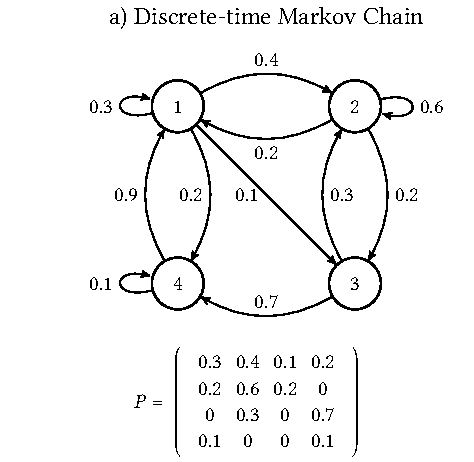
\includegraphics[width=0.5\linewidth]{Diagrams/mc_I/mc_I.pdf}}
	\subfloat{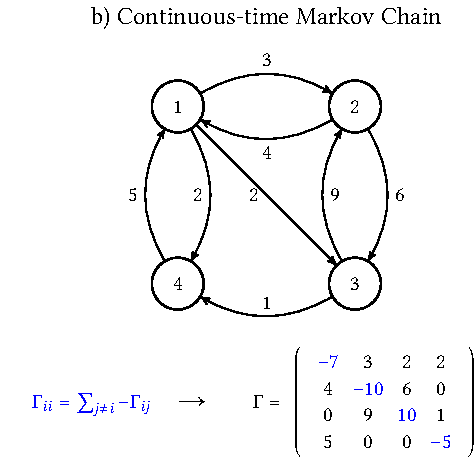
\includegraphics[width=0.5\linewidth]{Diagrams/mc_II/mc_II.pdf}}
	\caption[Discrete and continuous time Markov Chains.]{\textbf{Discrete and continuous time Markov Chains.} \textbf{left:} Discrete-time Markov Chain defined by $P$. \textbf{right:} Continuous-time Markov Chain defined by $\Gamma$.}
	\label{fig:mc-diagrams}
\end{figure}

\subsubsection{Continuous-time Markov Chains}
Defining a Markov chain in continuous time is slightly trickier as describing the system with a stochastic matrix does no longer suffice because transition probabilities become zero when considering an infinitesimal time. Instead a continuous-time Markov Chain (CTMC) is characterised by a \textbf{rate matrix} or \textbf{infinitesimal generator matrix} $\Gamma$ defined on the set $I$. A rate matrix has the following three properties
\begin{enumerate}[label=\roman*)]
	\item $0 \leq \Gamma_{ii} <\infty, \quad \forall i$
	\item $\Gamma_{ij} \geq 0, \quad \forall i \neq j$
	\item $\sum_{j \in I} \Gamma_{i j}=0, \quad \forall i$
\end{enumerate}
While the CTMC can be interpreted in a number of ways, we shall use the so called \textbf{jump chain} and \textbf{holding times} representation, see also Fig.~\ref{fig:holdingJumping}. 
\begin{figure}[h]
	\centering
	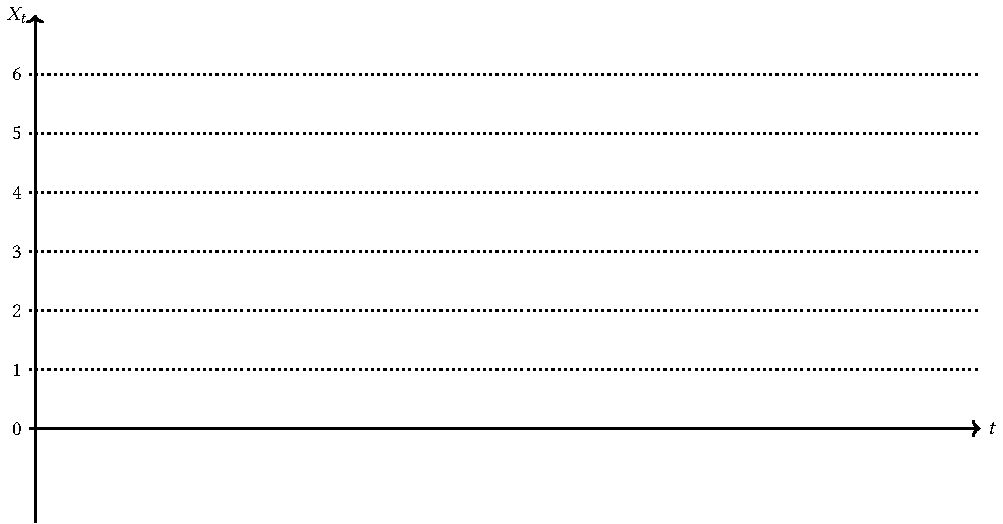
\includegraphics[width=\linewidth]{Diagrams/ctmc/ctmc}
	\caption[Jump chain and Holding times]{\textbf{Jump chain and Holding times.} A discrete space Markov process $\{X_t\}_{t\geq 0}$ in continuous time. The holding times $S_n$ are independent exponential random variables and the transition probabilities at jump times $J_n$ are given with the jump matrix $\Pi$. Inspired by~\cite{norris1998markov}.}
	\label{fig:holdingJumping}
\end{figure}
We can think of a CTMC as a series of discrete jumps, where the system remains in each state for a certain holding time. This suggests that we can construct the CTMC from a discrete-time chain with stochastic matrix $\Pi$, which we will call the \textbf{jump matrix}, and a set of independent random variables $\{S_n\}$ which determine the holding times. We construct matrix $\Pi$ by rescaling rows of $\Gamma$ so they add up to one, putting a $0$ on the diagonal
\begin{equation}
	\begin{array}{l}
		\Pi_{i j}=\left\{
		\begin{array}{ll}
			\Gamma_{i j} / \Gamma_{ii} & \text { if } j \neq i \text { and } \Gamma_{ii} \neq 0 \\
			 0 & \text { if } j \neq i \text { and } \Gamma_{ii}=0
		\end{array}\right. 
		\\ 
		\Pi_{i i}=\left\{
		\begin{array}{ll}
			0 & \qquad  \text { if } \Gamma_{ii} \neq 0 \\
			1 & \qquad \text { if } \Gamma_{ii}=0.
		\end{array}\right.
	\end{array}
\end{equation}
In order for the process to possess the Markov property, the distribution of holding times $\{S_n\}$ must be exponential~\cite{norris1998markov}, 
\begin{equation}
	S_{n+1} \sim \operatorname{Exp}(-{\Gamma_{ii}}(X_n)),
\end{equation}
with exponential parameters being $-\Gamma_{ii}$ where $i$ is the current state.
Processes with different holding time distributions are called \textbf{semi-Markov}. The jump times $\{J_n\}$ are simply 
\begin{equation}
	J_{n}=S_{1}+\ldots+S_{n}.
\end{equation}
\begin{definition}[Continuous-time Markov chain]
	A stochastic process $\{X_t\}_{t \geq 0}$ on set $I$ is a \textbf{continuous-time Markov chain} if its jump chain $\{Y_n\}_{n \geq 0}$ is a discrete-time Markov chain and its holding times $\{S_n\}_{n \geq 1}$ are independent exponential random variables $S_n \sim \operatorname{Exp}(-{\Gamma_{ii}}(X_n))$.
\end{definition}
An equivalent formulation is in terms of \textbf{competing exponentials}. Transitions $\Gamma_{j \rightarrow k}$ from $j$ to $k$ are defined as independent exponential random variables $\tau_{j \rightarrow k}$
\begin{equation}
	\tau_{j \rightarrow k} \sim \operatorname{Exp}(\Gamma_{jk}), \quad j \neq k
\end{equation}
the next state is then chosen as
\begin{equation}
	Y_{n+1} = \operatorname{argmin}_{k} \tau_{j \rightarrow k}.
\end{equation}
The chain $\{Y_n\}_{n\geq0}$ along with times 
\begin{equation}
	S_{n} = \min _{k} \tau_{j \rightarrow k},
\end{equation}
gives the full description of the CTMC. With this formulation in mind we now interpret $\Gamma_{ii}$ as the rate ob \emph{leaving} current state and $\Gamma_{i j}$ as the rate of \emph{going} from $i$ to $j$.

\section{The Feynman-Kac formula}
\label{subsec:fk-fk}
The Feynman path integral formulation~\eqref{eq:FPI} was extensively used by physicists for decades, even in the absence of a formal mathematical formulation which is hard to define because of the difficulties with defining an appropriate measure on the path space. Kac~\cite{kac1949distributions} provided a rigorous formulation of the \textit{real-valued} case of the Feynman path integral, and the resulting \emph{Feynman-Kac} formula provides a bridge between \emph{parabolic} partial differential equations and stochastic processes. 

To illustrate the Feynman-Kac formula let us consider a single particle with Hamiltonian
\begin{equation}
	\hat{H} = -\frac{\mathrm{d}^2~~}{\mathrm{d}x^2} + V(x)
\end{equation}
and the Schr\" odinger equation in \textit{imaginary time}, which is of the elliptic type, 
\begin{equation}
	\label{eq:imag_sch}
	\partial_t | \psi_t \rangle = - \hat{H} | \psi_t \rangle.
\end{equation}
Its formal solution, the time propagation of an initial wave function $|\phi_0\rangle$ at $t=0$, is written as
\begin{equation}
	\left| \psi_{t} \right\rangle = e^{-\hat{H} t}\left|\psi_{0}\right\rangle. 
\end{equation}
From the spectral decomposition of the operator $e^{-\hat{H} t}$ in terms of eigenstates $|\phi_n\rangle$ and eigen-energies $E_n$ of the Hamiltonian $\hat{H}$
\begin{equation}
	e^{-\hat{H} t}=\sum_{n} e^{-E_{n} t}|\phi_n\rangle\langle\phi_n|, 
\end{equation}
it follows that the term corresponding to the ground state of the system $|\phi_0\rangle$ decays the slowest. Thus starting in some initial state and propagating for a long imaginary time $it$ leads into the ground state with the decay rate giving the ground state energy as
\begin{equation}
	\lim_{t \rightarrow \infty} | \psi_t \rangle \propto e^{-E_0 t} | \phi_0 \rangle,
\end{equation} 
where $E_0$ is the ground state energy and $|\phi_0\rangle$ is the corresponding state. Kac noticed that the kinetic term of the Lagrangian in~\eqref{eq:FPI} could be interpreted as a measure on Brownian walks, and a solution to the imaginary time Schr\" odinger equation can be written as
\begin{equation}
	\psi(x, t)=\underset{X \sim \text { Brownian with } X_{t}=x}{\mathbb{E}}
	\left[\exp \left(-\int_{0}^{t}  V\left(X_{\tau}, \tau \right) \mathrm{d}\tau \right) \psi\left(X_{0}, 0\right)\right],
\end{equation}
where only the \textbf{endpoint} at time $t$ of the Brownian process fixed, whereas the starting point at time $t=0$ is not, $\psi (x, 0)$ encodes the initial condition into this representation. When there is no external potential $V(x) = 0$, the Schr\" odinger equation in imaginary time is the diffusion equation and the Feynman-Kac solution is simply
\begin{equation}
	\begin{aligned} 
		\psi(x, t) &= \underset{X \sim \text { Brownian with } X_{t}=x}{\mathbb{E}}\left[\psi\left(X_{0}, 0\right)\right] \\
		&=  
		\frac{1}{\sqrt{2 \pi t}} \int  e^{-\left(x-x^{\prime}\right)^{2} / 2 t} \psi_{0}\left(x^{\prime}\right) \mathrm{d} x^{\prime}
	\end{aligned}
\end{equation}
An illustration of the Feynman-Kac approach to the problem with no external potential $V(x)$ in 1D is depicted in Fig.~\ref{fig:fk_1d_example}.
\begin{figure}[h]
	\centering
	\subfloat
	{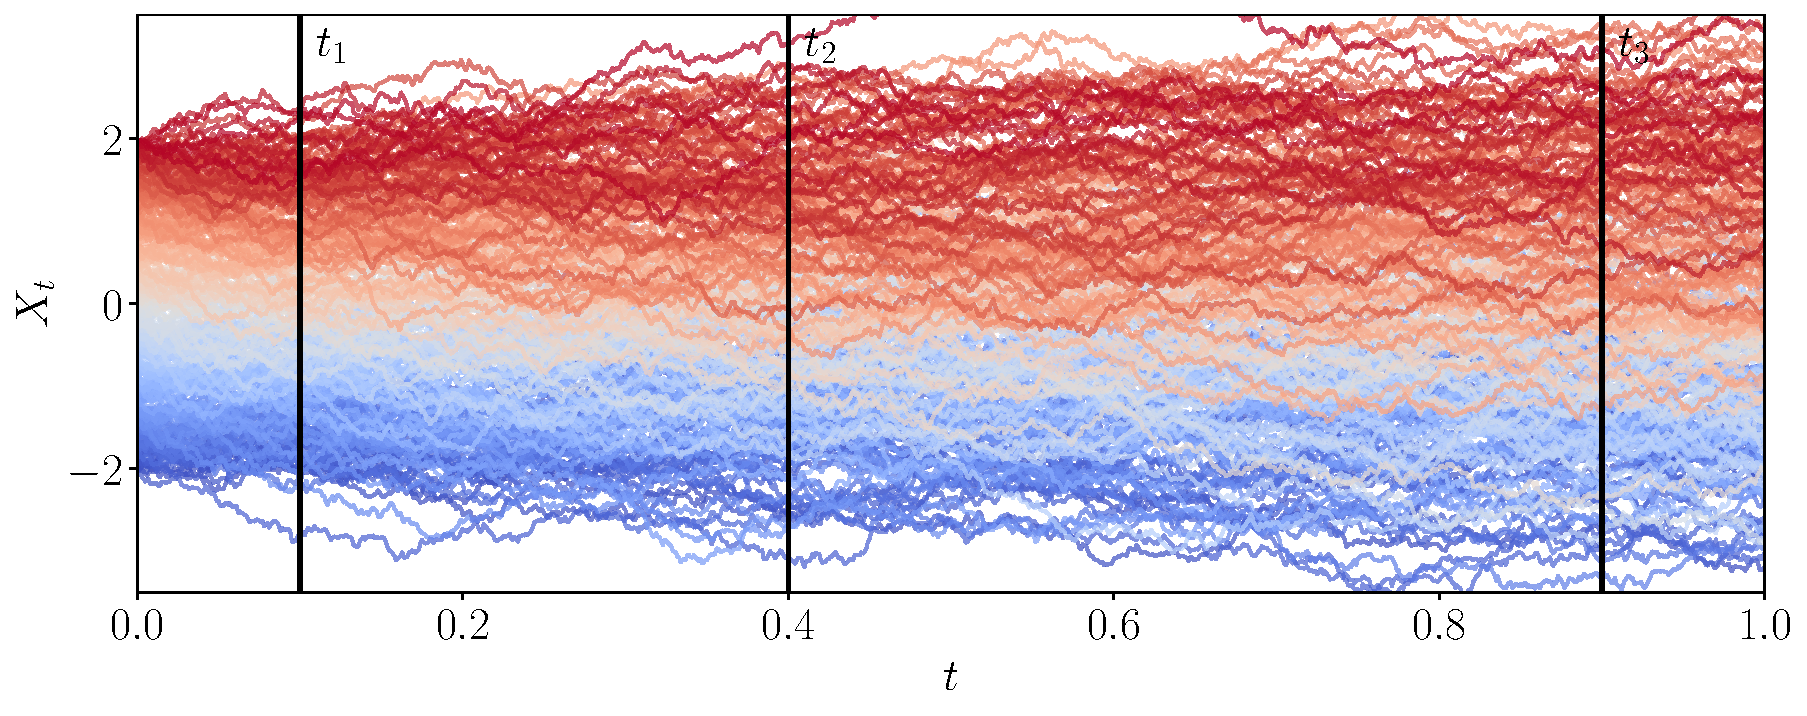
\includegraphics[width = \linewidth]{Chapter3/Figs/Raster/fkac_vs_fplanck_top.pdf}} \\
	\subfloat
	{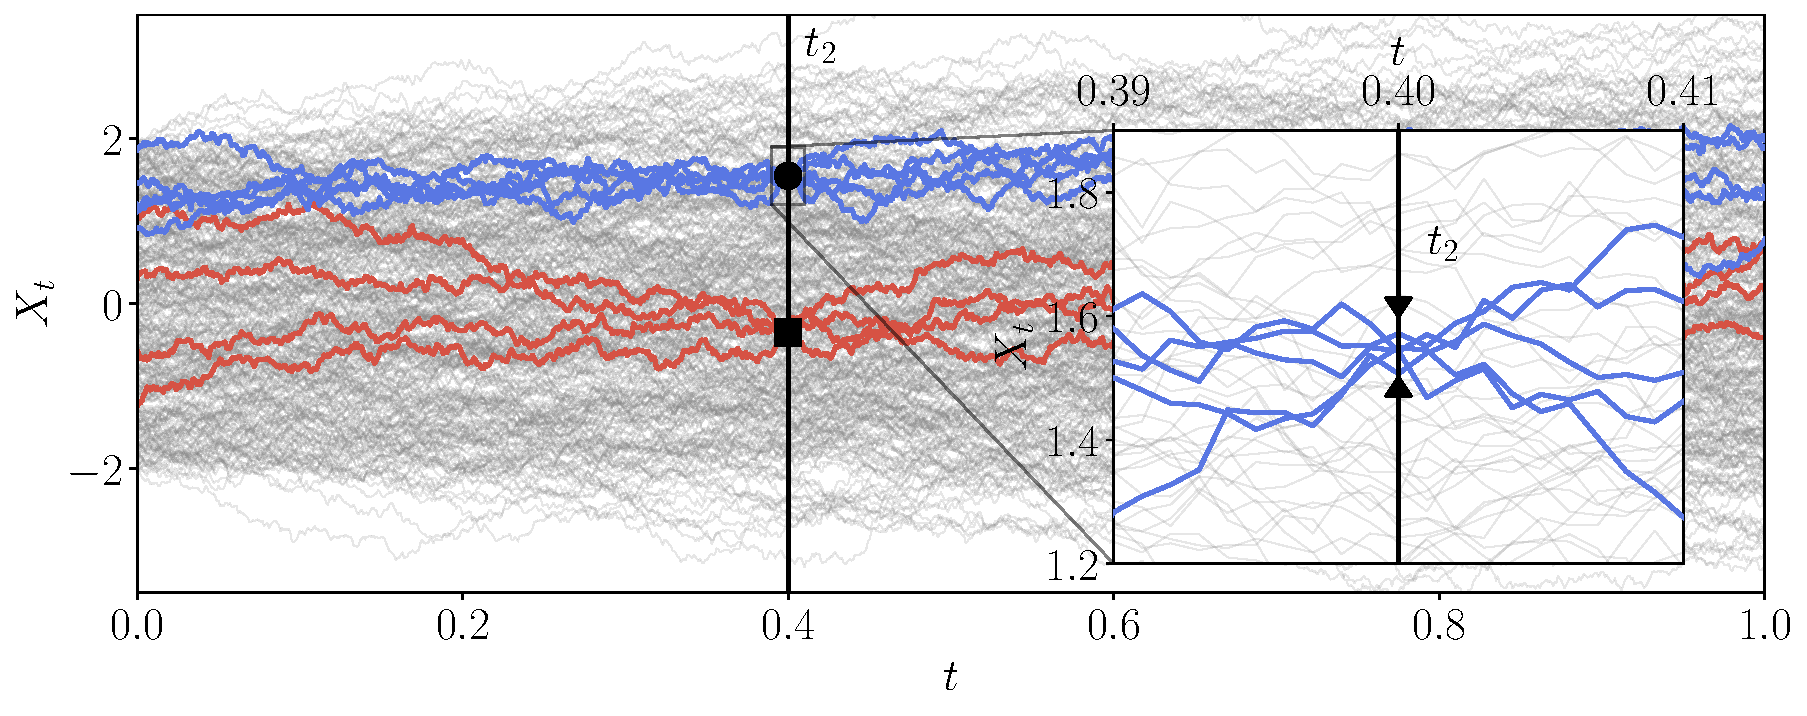
\includegraphics[width = \linewidth]{Chapter3/Figs/Raster/fkac_vs_fplanck_mid1.pdf}} \\
	\subfloat
	{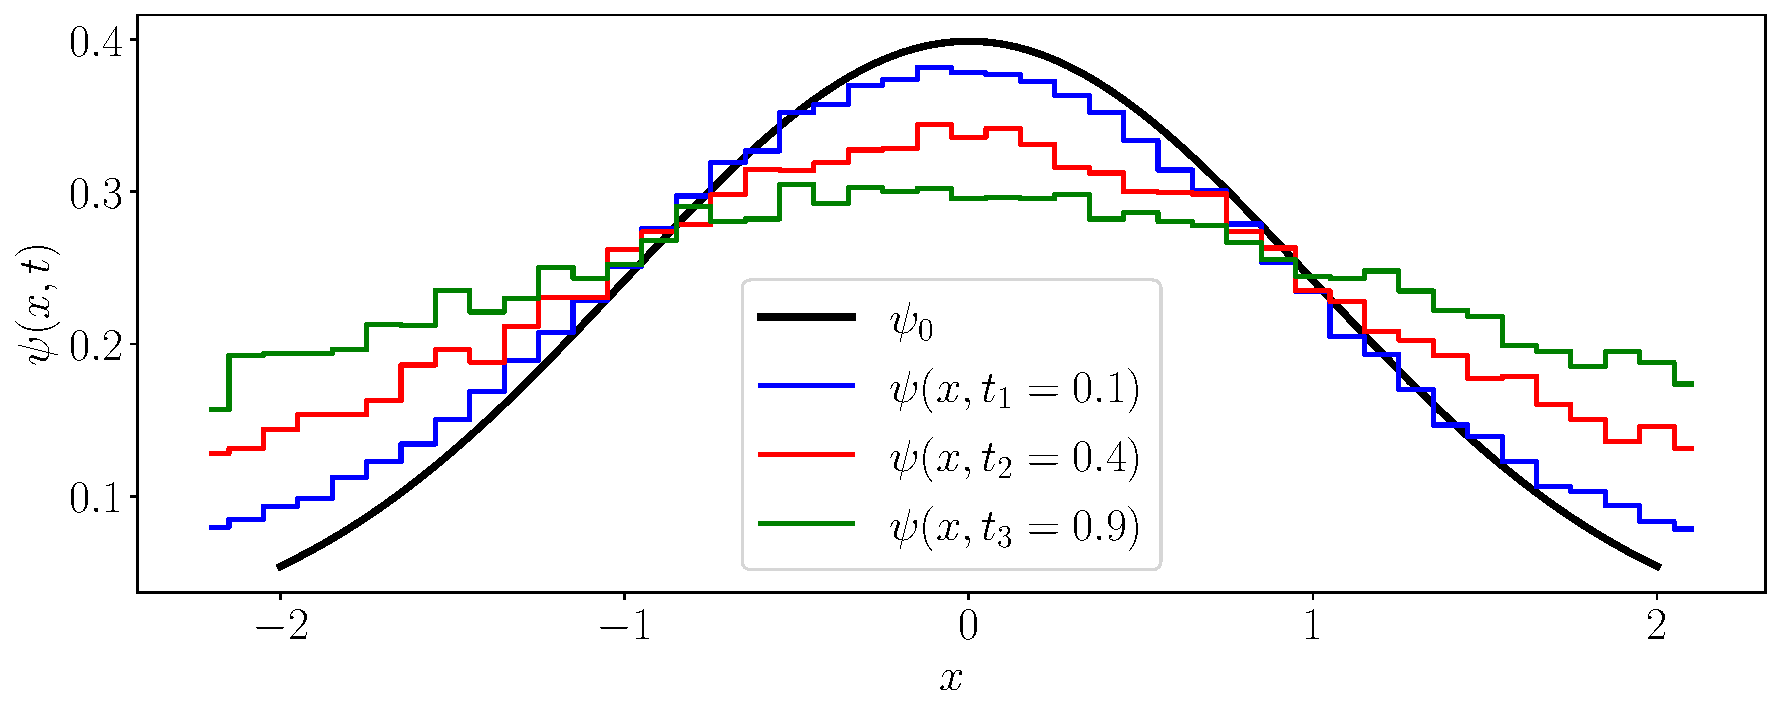
\includegraphics[width = \linewidth]{Chapter3/Figs/Raster/fkac_vs_fplanck_bottom.pdf}}
	
	\caption[Feynman-Kac for a free particle in 1D]{\textbf{Feynman-Kac for a free particle  in 1D.} \textbf{top:} $N=400$ Brownian walks starting from different $x_0$, the color signifies initial position. In order to evaluate $\psi$ between $x-\frac{\delta x}{2}$ and $x+\frac{\delta x}{2}$ at some time $t$ we must first find Brownian paths that end there. \textbf{middle:} The paths that pass through at $x \in (1.5, 1.6)$ (blue) and through $x \in (-0.4,-0.3)$ (red) are colored, others are left in grey. \textbf{bottom:} Time evolution of the initial condition $\psi_{0} = \frac{1}{\sqrt{2 \pi}} e^{-\frac{1}{2} x^{2}}$, by estimating ${\mathbb{E}}\left[\psi\left(X_{0}, 0\right)\right]$ from the filtered paths at each timestep.}
	\label{fig:fk_1d_example}
\end{figure}
This simple case, does not involve the potential $V(x)$. The role of the potential in the Feynman-Kac formula is to weight the Brownian paths, in turn defining the Feynman-Kac \emph{path measure} $\mathbb{P}_{\mathrm{FK}}$. A path measure is simply a measure on the path space and the Feynman-Kac measure is related to the Brownian measure $\mathbb{P}_{0}$ by the \emph{Radon-Nykodym} derivative
\begin{equation}
	\frac{\mathrm{d} \mathbb{P}_{\mathrm{FK}}}{\mathrm{d} \mathbb{P}_{0}}=\mathcal{N} \exp \left(-\int V\left(X_{t}\right) d t\right),
\end{equation}
where $\mathcal{N}$ is a normalizing constant. Intuitively we can understand the measure as assigning more weight to Brownian paths that spend more time in the attractive region ($V(x) < 0$) than in repulsive regions ($V(x) > 0$), this is illustrated in Fig.~\ref{fig:fkac_measure_reweight}.
\begin{figure}[H]
	\centering
	\subfloat{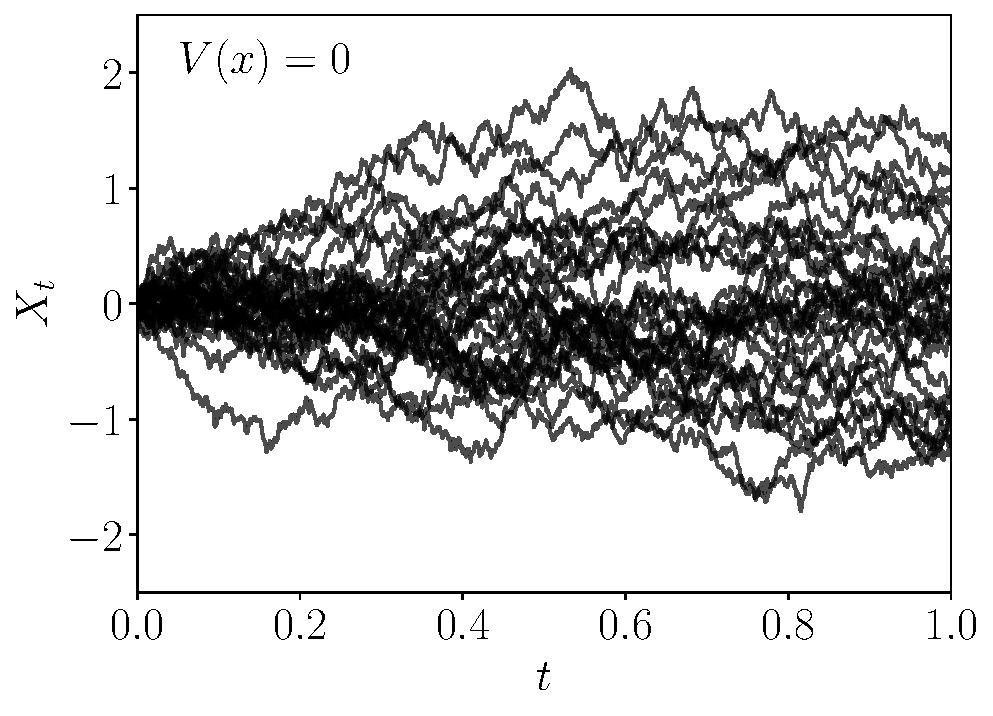
\includegraphics[width=0.5\linewidth]{Chapter3/Figs/Raster/reweight1.pdf}}
	\subfloat{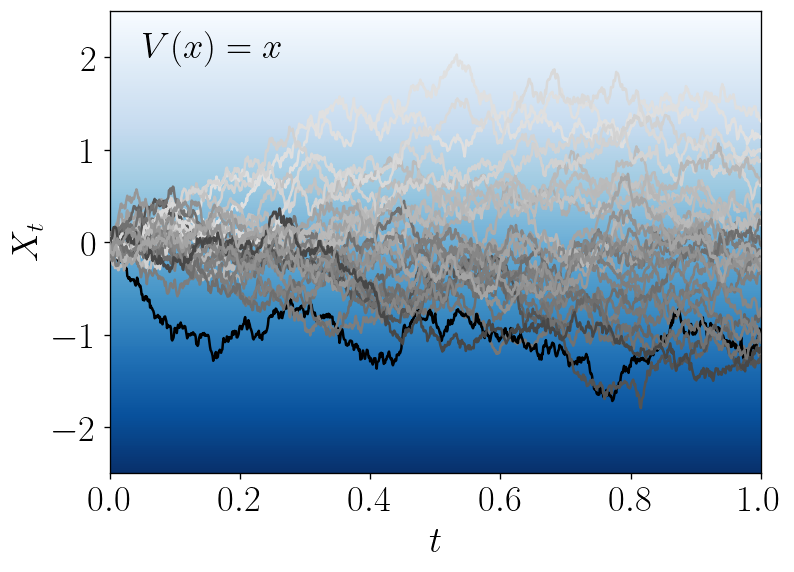
\includegraphics[width=0.5\linewidth]{Chapter3/Figs/Raster/reweight2.png}}
	\caption[Feynman-Kac measure in a linear potential]{\textbf{Feynman-Kac measure in a linear potential.} 
		\textbf{left:} $N=30$ Brownian paths. \textbf{right:} The paths colored by their likelihood under the Feynman-Kac measure with $V(x)=x$. }
	\label{fig:fkac_measure_reweight}
\end{figure}
Moreover, this new stochastic process is Markovian. This is crucial for our approach because of the connection with SDEs. In the continuous case we have discussed so far, the mapping between the Fokker-Planck equation and the Schr\" odinger equation is straightforward in terms of a similarity transform. Starting from the FP equation with drift $v(x)=-U^\prime(x)$ given as a gradient of some potential function $U(x)$ and its solution $\rho(t, x)$ 
\begin{equation}
	\frac{\partial \rho}{\partial t}=\mathcal{L}_{\mathrm{FP}} \rho=\frac{\partial}{\partial x}\left[\frac{\partial \rho}{\partial x}+U^{\prime}(x) \rho\right],
\end{equation}
we can define the function 
\begin{equation}
	\psi(x, t)=\frac{\rho(x, t)}{\sqrt{\rho_{0}(x)}},
\end{equation}
with $\rho_{0}$ being the stationary distribution of the FP equation
\begin{equation}
	\frac{\partial}{\partial x}\left[\frac{\partial \rho}{\partial x}+U^{\prime}(x) \rho\right] = 0 \quad \rightarrow \quad \rho_{0}(x) \propto \exp (-U(x)).
\end{equation}
Function $\psi(x, t)$ satisfies the imaginary time Schr\" odinger equation~\eqref{eq:imag_sch} with the Hamiltonian
\begin{equation}
	H=-\frac{\partial^{2}}{\partial x^{2}}-\frac{U^{\prime \prime}}{2}+\frac{U^{\prime 2}}{4}, 
\end{equation}
its ground state wavefunction is 
\begin{equation}
	\psi_{0}(x)=\sqrt{\rho_{0}(x)}.
\end{equation}
In other words, the quantum ground state probability distribution $|\psi_{0}|^2$ is the same as classical stationary distribution $\rho_{0}$ of the stochastic process $X_{t}$
\begin{equation}
	\mathrm{d} X_{t}=\mathrm{d} W_{t}+v\left(X_{t}\right) \mathrm{d} t,
\end{equation}
in the literature referred to as the \emph{Nelson's ground state process}~\cite{nelson1967dynamical, albeverio1977energy}. \hl{This connection serves as the backbone of our solution approach (revisit)}, as the ability to efficiently sample from the stochastic process is equivalent to sampling from the ground state of the quantum system. Even though the connection is simple, it comes with a caveat. Starting from the Schr\" odinger equation one needs to find the drift $v(x)$ and while the connection with the potential of the Hamiltonian is clear-cut in 1D, this is not the case in many-body systems, i.e. the \emph{inverse problem} of finding the stochastic process of a given Hamiltonian is difficult, and is one of the core problems approached in this thesis.

\newpage
\section{Stoquastic Hamiltonians and Lattice-model representations}
\label{subsec:fk-latt}
A similar connection between stochastic processes and the ground state exists in the discrete space, the difference being that instead of FP we have the Master equation


For a Markov process over discrete states, we can write the master equation as 
\begin{equation}
	\frac{\partial P_{j}}{\partial t}=\sum_{k \neq j}\left[\Gamma_{k \rightarrow j} P_{k}-\Gamma_{j \rightarrow k} P_{j}\right].
\end{equation}


%********************************** % ??? Section  *************************************
\newpage
\section{Quantum Mechanics, Control and loss functions}

\subsection{Continuous space}

\subsection{Discrete space}

\begin{figure}
	\centering
	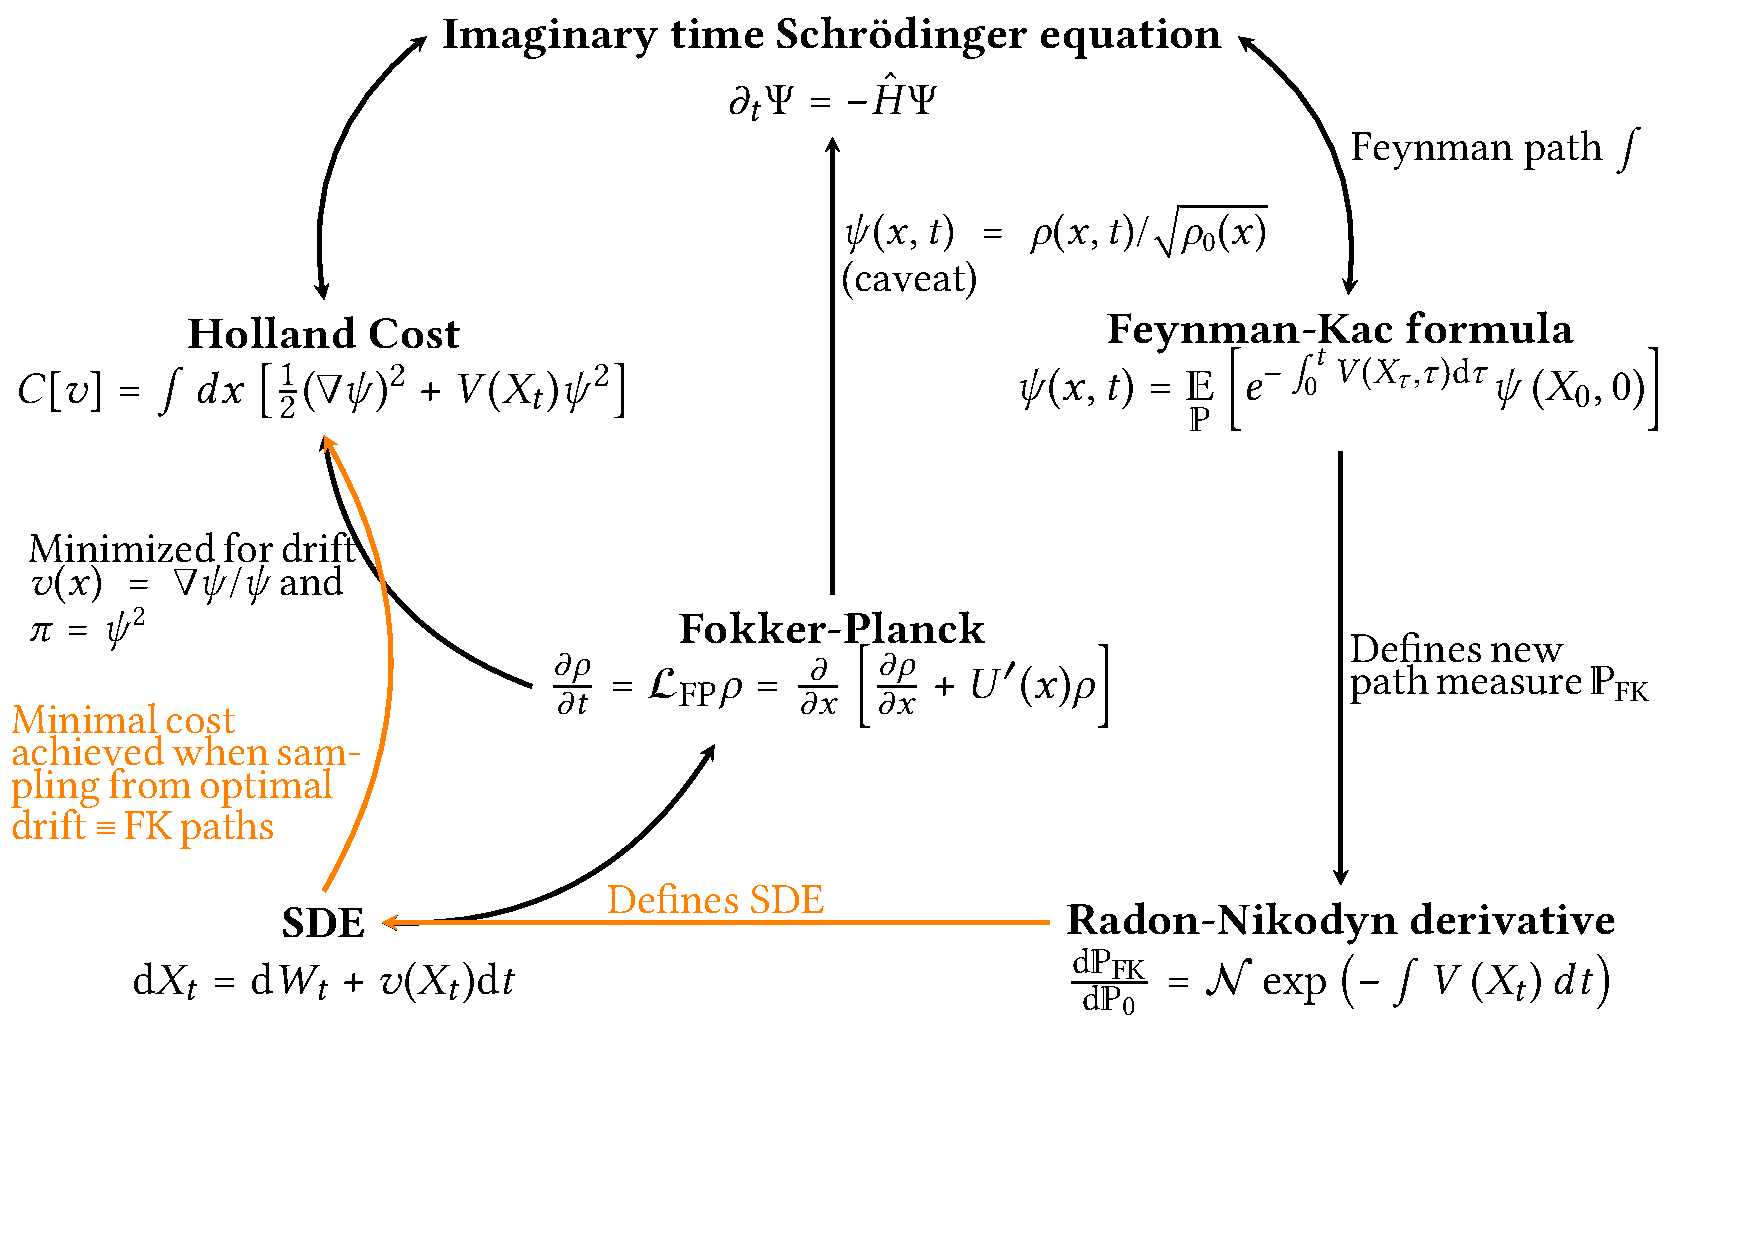
\includegraphics[angle=90, width=\linewidth]{Diagrams/bp/bp-c5.pdf}
	\caption[QM, stochastic processes and optimal control]{\textbf{QM, stochastic processes and optimal control}}
	\label{fig:bp-c5}
\end{figure}



%********************************** % Ch3 Nomenclature *************************************
\nomenclature[Z-sde]{SDE}{Stochastic Differential Equations}
\nomenclature[Z-RN]{RN}{Radon-Nikodym}
\nomenclature[Z-fp]{FP}{Fokker-Planck}
\nomenclature[z-pdf]{pdf}{Probability density function}
\nomenclature[z-cdf]{cdf}{Cumulative density function}
\nomenclature[z-stochprocs]{s.p.}{Stochastic process}
\nomenclature[z-dtmc]{DTMC}{Discrete time Markov Chain}
\nomenclature[z-ctmc]{DTMC}{Discrete time Markov Chain}

\nomenclature[x-ratematrix]{$\Gamma$}{Transition rate matrix}
\nomenclature[x-statespace]{S}{State space of a Markov process}
\nomenclature[x-reals]{$\mathbb{R}$}{The set of real numbers}
\nomenclature[x-normal]{$\mathcal{N}$}{The Gaussian distribution}
\nomenclature[x-measure]{$\mathbb{P}$}{Measure}
\nomenclature[x-filtration]{$\mathbb{F}$}{Filtration}
\nomenclature[x-field]{"$\mathcal{F}$"}{$\sigma$-field (algebra)}
\nomenclature[x-stochprocs]{$\{X_t\}$}{Stochastic process}
\nomenclature[x-randomvariable]{$\{X\}$}{Random variable}
\nomenclature[x-wiener]{$W_t$}{Wiener process, mathematical Brownian motion}
